\documentclass{article}
\usepackage{graphicx}
\graphicspath{{./figs/}}{}
\usepackage{listings}
\title{
HLS-Assignment 2.2
}
\begin{document}
\maketitle
\hfill \textbf{Sampath Govardhan} \\
\null \hfill \textbf{FWC22071}\\
\tableofcontents
\section{Problem Statement}
\begin{lstlisting}
Repeat the experiment in Assignment 2.1 with the following change:
Use arbitrary precision data type with bitwidth of 4 for integer and 24 
for fractional part of the inputs and figure out what the bitwidth of 
the output should be for your design.
\end{lstlisting}
\vspace{10cm}


\section{Design Code}
\begin{lstlisting}
#include <iostream>
#include "ap_fixed.h"

typedef ap_fixed<28,4> in;
typedef ap_fixed<56,8> out; \\maximum bitwidth of output will be 2*(24+4)

void mul(in a,in b,out &c)
{
 c = a * b;
}

\end{lstlisting}
\vspace{5cm}


\section{Test Bench Code}
\begin{lstlisting}
#include <iostream>
#include "ap_fixed.h"
using namespace std;

typedef ap_fixed<28,4> in;
typedef ap_fixed<56,8> out;


void mul(in a,in b,out &c);
int main()
{
in a;
in b;
out c;

int i;

for (i=0;i<=9;i++){
a = i+0.456789875;
b = i;
mul(a,b,c);
cout << "\n" << c;
}
return 0;
}


\end{lstlisting}
\vspace{5cm}


\section{C Simulation Output}
\begin{lstlisting}

INFO: [SIM 2] *************** CSIM start ***************
INFO: [SIM 4] CSIM will launch GCC as the compiler.
   Compiling ../../../../2.2/a2_2_tb.cpp in debug mode
   Generating csim.exe

0
1.45679
4.91358
10.3704
17.8272
27.2839
38.7407
52.1975
60.3457
45.8025
INFO: [SIM 1] CSim done with 0 errors.
INFO: [SIM 3] *************** CSIM finish ***************


\end{lstlisting}
\vspace{15cm}


\section{HLS Resource Consumption}
\vspace{3cm}
\begin{figure}[h]
    \centering
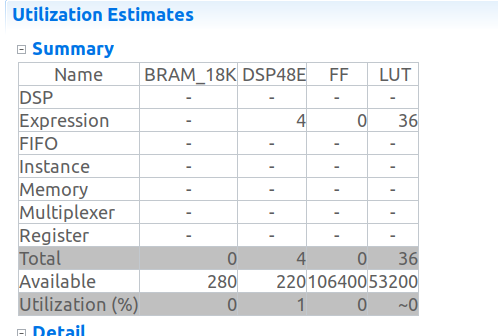
\includegraphics[width=\columnwidth]{figs/Resource_Consumption.png}
    \caption{Resource Consumption}
    \label{fig:my_label}
\end{figure}
\begin{lstlisting}
Here resourses used are more DSP's and LUT's compared to Assignment 2.1. 
This is because of using fractions, as computations of fractions are 
more complex compared to integers.
\end{lstlisting}
\vspace{5cm}


\section{HLS Timing Report}
\vspace{1cm}
\begin{figure}[h]
    \centering
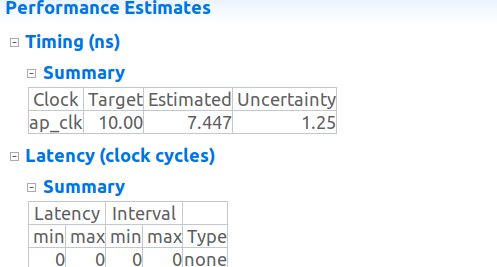
\includegraphics[width=\columnwidth]{figs/Timing_Report.png}
    \caption{Timing Report}
    \label{fig:my_label}
\end{figure}

\begin{lstlisting}
Here clock Uncertainity remains same but estimatd value is slightly less
compared to Assignment 2.1 this is because we are using 28 input bits 
and Assignment 2.1 uses 32 input bits also for each computation all bits 
are computed even if they are not used.
\end{lstlisting}
\vspace{10cm}


\section{Interfaces Report}
\vspace{1cm}
\begin{figure}[h]
    \centering
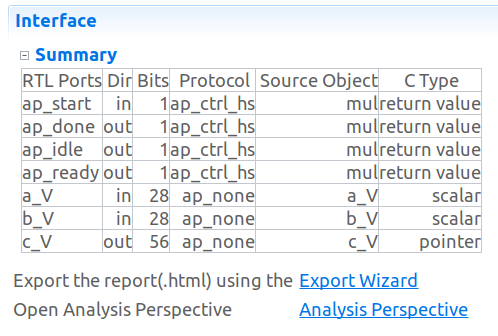
\includegraphics[width=\columnwidth]{figs/interfaces.png}
    \caption{Interface Summmary}
    \label{fig:my_label}
\end{figure}
\vspace{5cm}


\section{C/RTL Cosimulation Output}
\vspace{1cm}
\begin{lstlisting}


Starting C/RTL cosimulation ...
/tools/Xilinx/Vivado/2018.3/bin/vivado_hls /home/sam-admin/Xilinx-Vivado/HLS/Assignment2/a22/solution1/cosim.tcl
INFO: [HLS 200-10] Running '/tools/Xilinx/Vivado/2018.3/bin/unwrapped/lnx64.o/vivado_hls'
INFO: [HLS 200-10] For user 'sam-admin' on host 'sampaths-lappie' (Linux_x86_64 version 5.19.0-35-generic) on Fri Mar 17 18:32:10 IST 2023
INFO: [HLS 200-10] On os Ubuntu 22.04.2 LTS
INFO: [HLS 200-10] In directory '/home/sam-admin/Xilinx-Vivado/HLS/Assignment2'
INFO: [HLS 200-10] Opening project '/home/sam-admin/Xilinx-Vivado/HLS/Assignment2/a22'.
INFO: [HLS 200-10] Opening solution '/home/sam-admin/Xilinx-Vivado/HLS/Assignment2/a22/solution1'.
INFO: [SYN 201-201] Setting up clock 'default' with a period of 10ns.
INFO: [HLS 200-10] Setting target device to 'xc7z020clg484-1'
INFO: [COSIM 212-47] Using XSIM for RTL simulation.
INFO: [COSIM 212-14] Instrumenting C test bench ...
   Build using "/tools/Xilinx/Vivado/2018.3/tps/lnx64/gcc-6.2.0/bin/g++"
   Compiling a2_2.cpp_pre.cpp.tb.cpp
   Compiling a2_2_tb.cpp_pre.cpp.tb.cpp
   Compiling apatb_mul.cpp
   Generating cosim.tv.exe
INFO: [COSIM 212-302] Starting C TB testing ... 


0
1.45679
4.91358
10.3704
17.8272
27.2839
38.7407
52.1975
60.3457
45.8025INFO: [COSIM 212-333] Generating C post check test bench ...
INFO: [COSIM 212-12] Generating RTL test bench ...
INFO: [COSIM 212-323] Starting verilog simulation. 
INFO: [COSIM 212-15] Starting XSIM ...
INFO: [XSIM 43-3496] Using init file passed via -initfile option "/tools/Xilinx/Vivado/2018.3/data/xsim/ip/xsim_ip.ini".
Vivado Simulator 2018.3
Copyright 1986-1999, 2001-2018 Xilinx, Inc. All Rights Reserved.
Running: /tools/Xilinx/Vivado/2018.3/bin/unwrapped/lnx64.o/xelab xil_defaultlib.apatb_mul_top glbl -prj mul.prj -L smartconnect_v1_0 -L axi_protocol_checker_v1_1_12 -L axi_protocol_checker_v1_1_13 -L axis_protocol_checker_v1_1_11 -L axis_protocol_checker_v1_1_12 -L xil_defaultlib -L unisims_ver -L xpm --initfile /tools/Xilinx/Vivado/2018.3/data/xsim/ip/xsim_ip.ini --lib ieee_proposed=./ieee_proposed -s mul 
Multi-threading is on. Using 6 slave threads.
WARNING: [XSIM 43-3431] One or more environment variables have been detected which affect the operation of the C compiler. These are typically not set in standard installations and are not tested by Xilinx, however they may be appropriate for your system, so the flow will attempt to continue.  If errors occur, try running xelab with the "-mt off -v 1" switches to see more information from the C compiler. The following environment variables have been detected:
    LIBRARY_PATH
INFO: [VRFC 10-2263] Analyzing SystemVerilog file "/home/sam-admin/Xilinx-Vivado/HLS/Assignment2/a22/solution1/sim/verilog/glbl.v" into library work
INFO: [VRFC 10-311] analyzing module glbl
INFO: [VRFC 10-2263] Analyzing SystemVerilog file "/home/sam-admin/Xilinx-Vivado/HLS/Assignment2/a22/solution1/sim/verilog/mul.v" into library xil_defaultlib
INFO: [VRFC 10-311] analyzing module mul
INFO: [VRFC 10-2263] Analyzing SystemVerilog file "/home/sam-admin/Xilinx-Vivado/HLS/Assignment2/a22/solution1/sim/verilog/mul.autotb.v" into library xil_defaultlib
INFO: [VRFC 10-311] analyzing module apatb_mul_top
Starting static elaboration
Completed static elaboration
Starting simulation data flow analysis
Completed simulation data flow analysis
Time Resolution for simulation is 1ps
Compiling module xil_defaultlib.mul
Compiling module xil_defaultlib.apatb_mul_top
Compiling module work.glbl
Built simulation snapshot mul


****** Webtalk v2018.3 (64-bit)
  **** SW Build 2405991 on Thu Dec  6 23:36:41 MST 2018
  **** IP Build 2404404 on Fri Dec  7 01:43:56 MST 2018
    ** Copyright 1986-2018 Xilinx, Inc. All Rights Reserved.


source /home/sam-admin/Xilinx-Vivado/HLS/Assignment2/a22/solution1/sim/verilog/xsim.dir/mul/webtalk/xsim_webtalk.tcl -notrace
INFO: [Common 17-206] Exiting Webtalk at Fri Mar 17 18:32:53 2023...


****** xsim v2018.3 (64-bit)
  **** SW Build 2405991 on Thu Dec  6 23:36:41 MST 2018
  **** IP Build 2404404 on Fri Dec  7 01:43:56 MST 2018
    ** Copyright 1986-2018 Xilinx, Inc. All Rights Reserved.


source xsim.dir/mul/xsim_script.tcl
# xsim {mul} -autoloadwcfg -tclbatch {mul.tcl}
Vivado Simulator 2018.3
Time resolution is 1 ps
source mul.tcl
## run all
////////////////////////////////////////////////////////////////////////////////////
// Inter-Transaction Progress: Completed Transaction / Total Transaction
// Intra-Transaction Progress: Measured Latency / Latency Estimation * 100%
//
// RTL Simulation : "Inter-Transaction Progress" ["Intra-Transaction Progress"] @ "Simulation Time"
////////////////////////////////////////////////////////////////////////////////////
// RTL Simulation : 0 / 10 [n/a] @ "125000"
// RTL Simulation : 1 / 10 [n/a] @ "145000"
// RTL Simulation : 2 / 10 [n/a] @ "155000"
// RTL Simulation : 3 / 10 [n/a] @ "165000"
// RTL Simulation : 4 / 10 [n/a] @ "175000"
// RTL Simulation : 5 / 10 [n/a] @ "185000"
// RTL Simulation : 6 / 10 [n/a] @ "195000"
// RTL Simulation : 7 / 10 [n/a] @ "205000"
// RTL Simulation : 8 / 10 [n/a] @ "215000"
// RTL Simulation : 9 / 10 [n/a] @ "225000"
// RTL Simulation : 10 / 10 [n/a] @ "235000"
////////////////////////////////////////////////////////////////////////////////////
$finish called at time : 275 ns : File "/home/sam-admin/Xilinx-Vivado/HLS/Assignment2/a22/solution1/sim/verilog/mul.autotb.v" Line 328
## quit
INFO: [Common 17-206] Exiting xsim at Fri Mar 17 18:33:01 2023...
INFO: [COSIM 212-316] Starting C post checking ...


0
1.45679
4.91358
10.3704
17.8272
27.2839
38.7407
52.1975
60.3457
45.8025INFO: [COSIM 212-1000] *** C/RTL co-simulation finished: PASS ***
INFO: [COSIM 212-210] Design is translated to an combinational logic. II and Latency will be marked as all 0.
Finished C/RTL cosimulation.


\end{lstlisting}
\vspace{5cm}


\section{C/RTL Cosimulation Report}
\vspace{1cm}
\begin{figure}[h]
    \centering
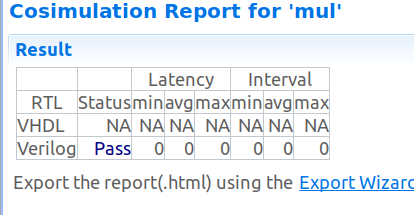
\includegraphics[width=\columnwidth]{figs/Cosim_report.png}
    \caption{Cosimulation Report}
    \label{fig:my_label}
\end{figure}
\end{document}
